\documentclass[tikz]{standalone}
\usetikzlibrary{arrows.meta,positioning,shapes.geometric,calc}
\begin{document}
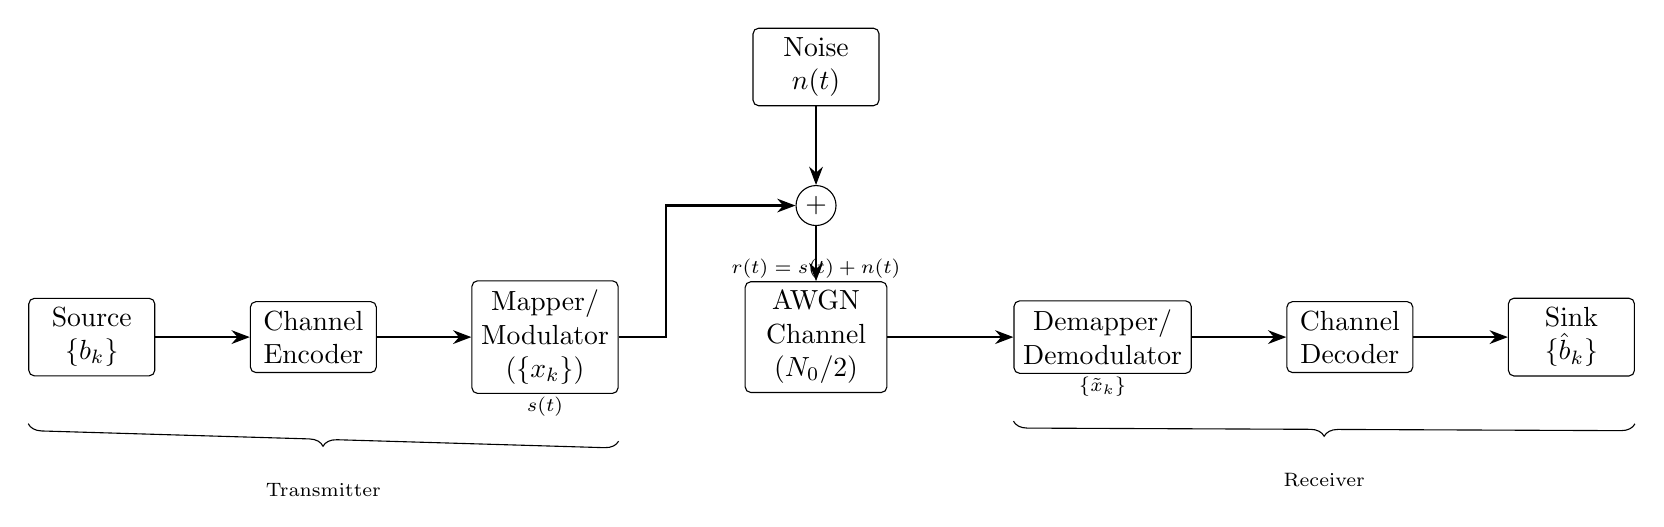
\begin{tikzpicture}[
  >=Stealth,
  block/.style = {draw, rounded corners=2pt, minimum height=9mm, minimum width=16mm, align=center},
  sum/.style   = {draw, circle, inner sep=1.5pt, minimum size=4mm},
  line/.style  = {->, thick},
  note/.style  = {font=\scriptsize, inner sep=1pt},
  node distance=10mm and 12mm
]
% Nodes
\node[block]            (src)   {Source\\$\{b_k\}$};
\node[block, right=of src] (enc)   {Channel\\Encoder};
\node[block, right=of enc] (mod)   {Mapper/\\Modulator\\($\{x_k\}$)};
\node[block, right=16mm of mod, minimum width=18mm] (chan)  {AWGN\\Channel\\($N_0/2$)};
\node[sum,  above=7mm of chan] (plus) {$+$};
\node[block, right=16mm of chan] (demod) {Demapper/\\Demodulator};
\node[block, right=of demod] (dec)   {Channel\\Decoder};
\node[block, right=of dec]   (sink)  {Sink\\$\{\hat b_k\}$};

% Noise source
\node[block, above=of plus] (noise) {Noise\\$n(t)$};

% Connections (TX path)
\draw[line] (src) -- (enc);
\draw[line] (enc) -- (mod);

% Channel: signal path via adder
\draw[line] (mod.east) -- ++(6mm,0) |- (plus.west);
\draw[line] (plus) -- (chan.north);

% Noise injection
\draw[line] (noise) -- (plus);

% RX path
\draw[line] (chan.east) -- (demod.west);
\draw[line] (demod) -- (dec);
\draw[line] (dec) -- (sink);

% Little annotations
\node[note, below=0mm of mod]   {$s(t)$};
\node[note, above=0mm of chan]  {$r(t)=s(t)+n(t)$};
\node[note, below=0mm of demod] {$\{\tilde x_k\}$};

% Decorative braces for TX/RX
\draw[decorate,decoration={brace,amplitude=5pt,mirror}] ($(src.south west)+(0,-6mm)$) -- node[below=6mm, note]{Transmitter} ($(mod.south east)+(0,-6mm)$);
\draw[decorate,decoration={brace,amplitude=5pt,mirror}] ($(demod.south west)+(0,-6mm)$) -- node[below=6mm, note]{Receiver} ($(sink.south east)+(0,-6mm)$);

\end{tikzpicture}
\end{document}
